\documentclass{article}
\usepackage[utf8]{inputenc}
\usepackage[english]{babel}
\usepackage{graphicx}
\usepackage{biblatex}
\usepackage{amssymb}
\usepackage{amsmath}
\usepackage{mathtools}
\usepackage{algorithm}
\usepackage[noend]{algpseudocode}
\usepackage{graphicx}
\usepackage{float}
\usepackage{scrextend}
\usepackage{hyperref}
\usepackage{caption}
\usepackage{subcaption}
 \usepackage{booktabs}
 \usepackage{enumerate}
\usepackage[table,xcdraw]{xcolor}
\usepackage{tikz}
\usetikzlibrary{matrix}
\usepackage{amsthm}

\newtheorem{theorem}{Theorem}[section]
\newtheorem{corollary}{Corollary}[theorem]
\newtheorem{lemma}[theorem]{Lemma}

\theoremstyle{definition}
\newtheorem{definition}{Definition}[section]


\newcommand{\Enc}{\texttt{Enc}}
\newcommand{\Dec}{\texttt{Dec}}
\newcommand{\Gen}{\texttt{Gen}}

\newcommand{\M}{\mathcal{M}}
\renewcommand{\C}{\mathcal{C}}
\newcommand{\K}{\mathcal{K}}
\newcommand{\A}{\mathcal{A}}
\renewcommand{\L}{\mathcal{L}}
\newcommand{\F}{\mathcal{F}}
\newcommand{\D}{\mathcal{D}}
\renewcommand{\P}{\mathcal{P}}

\newcommand{\Prob}{\mathbb{P}}

\newcommand{\Oh}{\mathcal{O}}

\newcommand{\Int}{\mathbb{Z}}
\newcommand{\Nat}{\mathbb{N}}
\newcommand{\Reals}{\mathbb{R}}
\renewcommand{\H}{\mathcal{H}}
\renewcommand{\vec}[1]{\textbf{#1}}

\newcommand{\PPT}{\texttt{PPT}}
\newcommand{\negl}{\text{negl}}
\renewcommand{\mod}{\,\,\text{mod}\,\,}

\newcommand{\Expr}[2]{\texttt{Expr}^{\texttt{#1}}_{#2}}
\newcommand{\Adv}[2]{\texttt{Adv}^{\texttt{#1}}_{#2}}

\newcommand{\norm}[1]{||#1||}

\addtokomafont{labelinglabel}{\sffamily}

\usepackage[a4paper, total={6in, 8in}]{geometry}

\addbibresource{dissertation.bib}

\title{CS4796: Joint Senior Honours Project}
\author{\{gf38\} @ st-andrews.ac.uk}

\makeatletter
\def\BState{\State\hskip-\ALG@thistlm}
\makeatother

\begin{document}

\begin{titlepage}
    \begin{center}
        \vspace*{1cm}
        
        \textbf{Fully homomorphic encryption}
        
        \vspace{0.5cm}
        
        CS4796: Joint Senior Honours Project \\
                
        
        \vspace{1cm}
        
        \textbf{Gergely Flamich}

        \vspace{0.5cm}
        Supervisors:\\
        Dr Sophie Huczynska, Prof Steve Linton
        
        \vfill
        
        
\includegraphics[width=0.5\textwidth]{img/uni_crest}
        
        \vspace{0.8cm}
        
        School of Computer Science\\
        University of St Andrews\\
        Scotland\\
        
    \end{center}
\end{titlepage}

\begin{abstract}
\end{abstract}
\paragraph{Declaration}
We declare that the material submitted for assessment is my own work except where credit is explicitly given to others by citation or acknowledgement. This work was performed during the current academic year except where otherwise stated. The main text of this project report is NN,NNN* words long, including project specification and plan. In submitting this project report to the University of St Andrews, I give permission for it to be made available for use in accordance with the regulations of the University Library. I also give permission for the report to be made available on the Web, for this work to be used in research within the University of St Andrews, and for any software to be released on an open source basis. I retain the copyright in this work, and ownership of any resulting intellectual property.

\newpage

\tableofcontents

\newpage


\section{Introduction}
\paragraph{}
Cryptography is a fascinating subject, not only because it occupies the gray
zone between pure mathematics and computer science, but also because of how much
and how diversely it draws from both disciplines. It is a subject that has its
roots going back as far as the beginning of human communications. Regarded
for most of history as an art, but certainly a very intuition-based and ad hoc
discipline, during the 20th century it has transformed into a precise mathematical
science throught the works of Shannon \cite{shannon1949communication}, later Diffie and Hellman
\cite{diffie1976new} and Rivest, Shamir and Adleman \cite{rivest1978method}
kicking off the public-key revolution.
\paragraph{}
Fully homomorphic cryptosystems - one of which is the topic of is this work - are one
of the many fruits that this transformation has enabled. These schemes are such
that, in some sense, they do not only allow the encryption of data but also
arbitrary computations as well. Such a scheme in theory allows any concievable
program to be encrypted and ran on some untrusted party, without reavealing
enough information that any adversary could learn what is being computed.
\paragraph{}
It is not possible to present every, in itself marvellous, aspect of these
cryptosystems. Nonetheless, the author hopes to present the key ideas as
clearly and in as self-contained of a manner as possible. Where it is not
possible to advance without significant deviation from the topic, the
appropriate citation will be given to the external result.
\paragraph{}
This work is divided into three parts: \textbf{the first half} of this text is an
introduction to/ survey of the mathematical and computer scientific foundations
upon which the second half is built. \textbf{The second half} of this text will
detail the cryptosystem invented by Gentry, published in 2009
\cite{gentry2009fully}. \textbf{Finally}, the text is accompanied by a
collection of \texttt{Sage} \cite{SageMath} programs. They are implementations
of the schemes presented below and they are aimed to illuminate the practical
aspects of their respective cryptosystem.

\section{Mathematical Preliminaries}
\paragraph{}
Throughout this work some basic concepts will be used, the most important of
which will be given below.
\begin{definition}{Strings over an alphabet:}
  Let $A$ be a finite set of symbols, called an \textbf{alphabet} the strings
  over $A$ denoted $A^*$ is the set of all finite length sequences of
  symbols from $A$, including $\epsilon$, the empty string. Formally:
  \[
    A^* = \bigcup_{n\in \Nat \cup \{0\}} A^n.
  \]
  Here $\epsilon = () \in A^0$, the empty tuple. When talking about strings from $A^*$, instead of $s = (a_1, a_2, \hdots, a_n)
  \in A^*$, we will just write $a_1a_2\hdots a_n$.
\end{definition}
\paragraph{}
A natural property of strings is their length, i.e. the number of symbols they
are composed of. Thus, let $|\cdot| : A
\mapsto \Nat \cup \{0\}$ be defined as
\[
  \forall s \in A^* \quad |s| = n \Leftrightarrow s \in A^n
\]
\paragraph{}
A natural operation on strings is concatentaion. Formally, let $A$ be an
alphabet. Then, let $+ : A^* \times A^* \mapsto A^*$, such that
\[
  \forall s_1 = a_1\hdots a_n, s_2 = b_1 \hdots b_m \in A^*.\quad s_1 + s_2 =
  a_1\hdots a_nb_1 \hdots b_m \in A^*.
\]
\begin{definition}{Group:}
  Let $G$ be a non-empty set and $\circ: G \times G \mapsto G$ a binary operation on $G$.
  Then we will say that $(G, \circ)$ is a group if the following axioms hold:
  \begin{itemize}
  \item \textbf{G1:} $\forall a, b, c \in G$ we have $(a \circ b) \circ c = a
    \circ (b \circ c)$. (associativity)
  \item \textbf{G2:} $\exists 1 \in G. \,\forall a \in G$ we have $1 \circ a = a \circ 1 = a.$ (existence of an identity)
    \\
    It is easy to show that if such an element $1$ exists, then it
    is unique. We will call this unique element the \textbf{identity} of $G$.
    
  \item \textbf{G3:} $\forall a \in G\, \exists a^{-1} \in G$ such that $a \circ
    a^{-1} = a ^{-1} \circ a = 1$. (existence of inverses)
    \\
    It is easy to show that if this axiom holds
    then for every $a$ the corresponding $a^{-1}$ is unique. We will call this
    unique element the \textbf{inverse} of $a$. 
  \end{itemize}
\end{definition}
\paragraph{} If $G$ is finite, we call ($G, \circ$) a \textbf{finite group}.
\begin{definition}{Big-O notation:} Let $f, g: \Nat \mapsto \Reals $ be
  functions. Then we will write
  \[
    f(n) = \Oh(g(n)) \quad \text{(and say $f$ is of order big oh of $g$)}
  \]
  if and only if
  \[
    \exists M \in \Reals. \exists N \in \Nat.\quad \forall n \geq N \Rightarrow
    |f(n)| \leq M|g(n)|.
  \]
  Intuitively, this means that $f$ grows \textbf{at most} as fast as $g$.
\end{definition}
\section{A Very Brief History of Ciphers}
\paragraph{}
The history of ciphers goes back at least 2000 years. We will now examine the
cipher now named after Julius Ceasar, who used the following method to obfuscate
his correspondance for his adversaries:
\paragraph{Ceasar Cipher}: Take the message (written using symbols from the
Latin alphabet) that we wish to obfuscate. Replace each symbol with the one that
comes 3 places after it in the alphabet. For letters at the end where we could
not shift, we ``wrap around'' to the beginning of the alphabet and carry on
counting from there. For example
\[
  \textit{Alea iacta est} \quad\to\quad \textit{Dohd mdfzd hxz}.
\]
To decrypt a message, we simply shift backwards by 3 positions, e.g.
\[
  \textit{Zhqm, zmgm, zmgm} \quad\to\quad \textit{Veni, vidi, vici}.
\]
\paragraph{}
We can further generalise this concept to arrive at the definition of
\textit{shift ciphers}, where instead of the fixing the shift to 3, we pick a
key $k \in \mathbb{N}$, and we then shift $k$ places forward (and backwards).
With shift ciphers in mind, we now formally defined some key concepts that will
be used throughout this work.
\begin{definition}{Cipher:}
  Let $\M, \C, \K_\Enc, \K_\Dec$ be alphabets. We will refer to $\M$
  as the \textbf{message space} and to $\C$ as the \textbf{cipher space}.
  A cipher $C$ over $\M$, $\K_\Enc$ and $\K_\Dec$ is a tuple $(\Gen, \Enc, \Dec)$, where
  \begin{itemize}
  \item $\Gen$ is the \textbf{key generation algorithm}, which outputs a key
    $(k_\Enc, k_\Dec) \in (\K_\Enc^* \times \K_\Dec^*)$, chosen according to some
    distribution. We refer to the set $\K\subseteq \K_\Enc^* \times \K_\Dec^*$ of all possible outputs of $\Gen$ as the
    \textbf{key space} of $C$. If for all outputs there is a polynomial time
    function $f$ such that $f(k_\Enc) = k_\Dec$, then we call $C$
    a \textbf{symmetric cipher} and instead of the tuple we just write $k$.
    Otherwise we call $C$ an \textbf{asymmetric cipher}.
    Since $\Gen$ is usually a probabilistic algorithm, we will denote generating
    its output by $k \leftarrow \Gen$ instead of $k = \Gen$ to emphasize the
    randomised nature of the function.
  \item $\Enc: \K_\Enc^*\times\M\mapsto \C$ is the \textbf{encryption algorithm}, which takes
    a encryption key $k$ and a message $m$ and outputs its encoding $c$. We will often
    refer to the message as the \textbf{plaintext} and to the encrypted message
    as \textbf{ciphertext}.
    \paragraph{Note:} $\Enc$ is not necessarily deterministic. When it is
    probabilistic, we will write $c \leftarrow \Enc_k(m)$ instead of $c = \Enc_k(m)$.
  \item $\Dec: \K_\Dec^*\times\C \mapsto \M$ is the \textbf{decryption algorithm}, which
    takes some decryption key $k$ and some ciphertext $c$ and outputs its
    correspnding plaintext $m$. 
    \paragraph{Note:} $\Dec$ is \textbf{always} deterministic (otherwise the
    scheme could never be assumed to be correct).
  \end{itemize}
  Finally, we require the correctness of $C$, concretely
  \[
    \forall m \in \M, \forall (k, k') \in \K. \quad \Dec(k', \Enc(k, m)) = m,
  \]
  i.e. that the cipher does not change its contents.
\end{definition}
\paragraph{Note:} For classical ciphers, we usually consider $\M = \C$ to be the
English (or Latin) alphabet. For modern crypto systems we will always work with
bitstrings, i.e. $\M$, $\C$ and $\K$ will be some subset of $\{0, 1\}^*$.
\paragraph{Equivalences of alphabets}
Consider any alphabet $\M = \{m_1, \hdots m_n\}$. It will be 
often convenient to consider the encoding of such an alphabet as something that
may be studied and manipulated more easily. Formally, by an encoding we mean a
bijection $f$ between our alphabet and some other set, where calculating values
of $f$ and $f^{-1}$ can both be done in polynomial time. Such an encoding may
be using ASCII for characters of the English alphabet or associating some
symbols with the elements of $\Int_n$. If there is such a bijection between
two alphabets, since one can be efficiently transformed into the other, we will
consider them equivalent.

\paragraph{Example}
Let us now revisit shift ciphers. In this case, for a set of $n$ symbols, it
will be easier to consider the encoding as elements of the additive group
$\Int_n$. First, it is easy to see that we are dealing with a
symmetric cipher, and since a shift by $k$ and any $k + xn, x \in \mathbb{N}$ is
going to be the same, $\K = \Int_n$. Then,
\begin{itemize}
\item $\Gen$: $\Gen$ is uniformly picking an element from $\Int_n$.
\item $\Enc$: We note that if we relabel our symbols to their
  indices (i.e. $m_i \to i$), then we can express our encryption function as
  \[
    \Enc(k, i) = i + k \mod n.
  \]
\item $\Dec$: Similarly, performing the above relabeling, we get
  \[
    \Dec(k, i) = i - k \mod n.
  \]
\end{itemize}
Now, checking the correctness of $C_{shift}$: Let $k, m \in \Int_n$
\[
  \Dec(k, \Enc(k, m)) = m + k \mod n - k \mod n = m + k - k \mod n = m \mod n = m.
\]
Since $k$ and $m$ were arbitrary, it holds $\forall m, k \in \Int_n$.
\paragraph{Kerckhoffs' principle}
Throughout the history of cryptography it has become evident that one must not
rely on the assumption that the adversary cannot obtain every detail about one's
crypto-system. This lead to the following important guiding principle in the
design of new schemes:
\begin{quotation}
The security of a scheme must lay in the key and not the scheme.
\end{quotation}
\section{Perfect Security}
In order for us to be able to analyse our schemes, we must have two well defined
notions: what does it mean that a scheme is \textit{secure} and how \textit{powerful} is
the adversary who wishes to break our scheme.
\paragraph{The adversary} We will start from a rather
paranoid, but very useful perspective: we will assume that the adversary has
unbounded computational power. This means that we will have to fend off attacks
that may involve computing arbitrary \textit{decidable} functions, no matter how
long they take to calculate. Also, by Kerckhoff's principle we assume that the
adversary has perfect knowledge of both our encryption and decryption functions.
\paragraph{Security} We will also impose a very stringent constraint on what we
consider secure.
\begin{definition}{Perfect Security}
  \label{def:perfect_security}
We say that a scheme $\Pi$ is perfectly secure if
\[
  \forall m \in \M, c \in \C.\quad \Prob(M=m \,|\, C=c) = \Prob(M=m).
\]
\end{definition}
\paragraph{Indistinguishability} We will require that given any ciphertext and a uniformly
random string from the cipher alphabet, the adversary cannot
\textit{distinguish} the two strings whatsoever. To formalise this, we will
first need to define a \textbf{security experiment}:
\paragraph{}
Let $\Pi = (\Gen, \Enc, \Dec)$ be a scheme, and $\A$ be any adversary.
Then, we will define $\texttt{Expr}^{\texttt{eav}}_{\Pi, \A}$ as
follows:
\begin{enumerate}
\item $\A$ generates two messages $m_0$ and $m_1$ from the message space $\M$.
\item A random bit $b$ is chosen from $\{0, 1\}$.
\item Put $k \leftarrow \Gen()$ and $c = \Enc_k(m_b)$.
\item $\A$ is given $c$, and outputs $b'= \{0, 1\}$
\item The experiment outputs 1 if $b = b'$ and write $\Expr{eav}{\A, \Pi} = 1$,
  and 0 otherwise. If the output is 1, we say that $\A$ \textbf{succeeds}.
\end{enumerate}
Now, we are ready for our first definition of security:
\begin{definition}{Perfect Indistinguishability}
  \label{def:perfect_indistinguishability}
We say that a scheme $\Pi$ is perfectly indistinguishable iff for all adversaries $\A$
\[
  \Prob(\Expr{eav}{\A, \Pi} = 1) = \frac12.
\]
\end{definition}
\begin{theorem}
  \label{thm:perfect_equivalence}
A scheme $\Pi$ is perfectly secure if and only if it is perfectly indistinguishable.
\end{theorem}
\begin{proof}
  `$\Rightarrow$' Let $\A$ be an arbitrary adversary. Without loss
  of generality, we may assume that $\A$ outputs $m_0, m_1$ and that $\Gen$
  outputs $k$. Let $c_0 = \Enc_k(m_0)$ and $c_1 = \Enc_k(m_1)$. Then,
  \begin{align*}
    \Prob(\Expr{eav}{\A, \Pi} = 1) &= \Prob(\A \,\text{outputs 0}\,| B = 0)\Prob(B = 0) + \Prob(\A \,\text{outputs 1}\,| B = 1)\Prob(B = 1) \quad\text{by definition}\\
    &= \frac12\Prob(\A \,\text{outputs 0}\,| B = 0) + \frac12\Prob(\A \,\text{outputs 1}\,| B = 1)
  \end{align*}
  Notice, that since $B$ completely determines whether we have receive $c_0$ or
  $c_1$, we have $\Prob(B = b) = \Prob(C = c_b)$. Letting
  $\Prob(\A\,\text{outputs 0} | C = c_0) = p$ and $\Prob(\A\,\text{outputs 1} |
  C = c_1) = q$, we get
  \begin{equation}
    \begin{split}
    \label{eq:perfequivforward}
    \Prob(\Expr{eav}{\A, \Pi} = 1) &= \frac12 \Prob(\A \, \text{outputs 0} \,| C = c_0) + \frac12 \Prob(\A \,\text{outputs 1}\,| C = c_1) \\
                                   &= \frac12 p + \frac12 q \\
                                   &=  \frac12 (p + q)
    \end{split}
  \end{equation}
  Recall that since $\Pi$ is perfectly secure, $\forall m \in \M$ and $\forall c
  \in \C$ we have $\Prob(M = m | C = c) = \Prob(M = m)$. In particular, we have
  \[
    \Prob(M = m_0) = \Prob(M = m_0 | C = c_0) = \Prob(M = m_0 | C = c_1).
  \]
  Note, that beside the complete knowledge of the system the \textbf{only information} $\A$
  may work with is the value of $C$ to infer anything about the value of $M$.
  It is clear from above, that the knowledge of the value of $C$ does not change
  the amount of information that can be inferred about the value of $M$.
  Therefore, $\A$ must treat $c_0$ and $c_1$ the same way and so the probability that $\A$ guesses $0$ correctly must be equal to when $\A$ guesses
  $0$ incorrectly! Formally:
  \[
    \Prob(\A \, \text{outputs 0} \,| C = c_0) = \Prob(\A \,
    \text{outputs 0} \,| C = c_1) = p.
  \]
  and from this, we get
  \[
  q = \Prob(\A \, \text{outputs 1} \,| C = c_1) =
  1 - \Prob(\A \, \text{outputs 0} \,| C = c_1) = 1 - p.
  \]
  Combining this with Equation \ref{eq:perfequivforward}, we have
  \[
    \Prob(\Expr{eav}{\A, \Pi} = 1) = \frac12 (p + q) = \frac12 (p + 1 - p) = \frac12.
  \]
  `$\Leftarrow$' We shall prove this direction through a contradiction. Thus,
  assume $\Pi$ is not perfectly secure. Then, it is easy to see the following:
  \paragraph{Claim:} $\exists m \in \M$ for which $\exists c_0, c_1 \in \C$ such
  that
  \[
    \Prob(M = m | C = c_0) \neq \Prob(M = m | C = c_1).
  \]
  \paragraph{} To see this, assume the opposite: $\forall m \in \M, \forall c
  \in \C$ we have $\Prob(M = m | C = c) = p$ for some $p \geq 0$. Since $\Pi$ is
  not perfectly secure, $\exists m \in \M. \exists c \in \C$ such that
  \[
    \Prob(M = m) \neq Prob(M = m | C = c) = p.
  \]
  But then,
  \begin{align*}
    \Prob(M = m) &= \sum_{c' \in \C} \Prob(M = m | C = c')\Prob(C = c') \\
                 &= \sum_{c' \in \C} p\Prob(C = c')\quad\text{by our assumption above} \\
   &= p\sum_{c' \in \C} \Prob(C = c') = p.
  \end{align*}
  This violates our assumption that $\Pi$ is not perfectly secure, so the claim
  must hold.
  \paragraph{}
  Let $m \in \M$, $c_0, c_1 \in \C$ be as in the above claim. Without loss of
  generality, we may assume, that
  \[
    \Prob(M = m | C = c_0) = \Prob(M = m | C = c_1) + \delta
  \]
  where $\delta > 0$. Now, construct the following adversary $\A$:
  \begin{enumerate}
    \item $\A$ outputs $m_0 = m$ and some other arbitrary $m_1 = m'$.
    \item When $\A$ receives $c_0$ output $0$, $1$ when it receives $c_1$ and
      output a uniformly random guess otherwise.
  \end{enumerate}
  Note that the probability in any case that $\A$ guesses 0 correctly is the
  probabilty that $\A$ guesses 0 given the ciphertext multiplied by the
  probability that given the ciphertext the underlying message is $m_0 = m$.
  Therefore, the probability that $\A$ outputs $0$ given $B = 0$ is
  \begin{align*}
    \Prob(\A \, \text{outputs 0} | B = 0) &= \sum_{\substack{c \in \C \\ c \neq c_0, c_1}} \Prob(\A \, \text{outputs 0} | C = c)\Prob(M = m | C = c) + \Prob(\A \, \text{outputs 0} | C = c)\Prob(M = m | C = c_0) \\
                                          &\quad\quad\quad+ \Prob(\A \, \text{outputs 0} | C = c_1)\Prob(M = m | C = c_1)\\
                                          &= \sum_{\substack{c \in \C \\ c \neq c_0, c_1}} \frac12\Prob(M = m | C = c) + \Prob(M = m | C = c_0)\\
                                          &= \frac12 \sum_{\substack{c \in \C \\ c \neq c_0, c_1}} \Prob(M = m | C = c) + \Prob(M = m | C = c_0)\\
    \end{align*}
    Adding and taking away the missing terms in the sum, we have
    \begin{align*}
      \Prob(\A \, \text{outputs 0} | B = 0) &= \frac12\sum_{c \in \C} \Prob(M = m | C = c) + \frac12\left(\Prob(M = m | C = c_0) - \Prob(M = m | C = c_1)\right) \\
                                            &= \frac12 + \frac{\delta}{2} = p
  \end{align*}
  Similarly, we get $q = \frac12 + \frac{\delta}{2}$. Hence, by Equation
  \ref{eq:perfequivforward} we have
  \[
    \Prob(\Expr{eav}{\Pi, \A} = 1) = \frac12 (p + q) = \frac12 (\frac12 +
    \frac{\delta}{2} + \frac12 + \frac{\delta}{2}) = \frac12 + \frac{\delta}{2}.
  \]
  Hence $\Pi$ is not perfectly indistinguishable. Since the contraposition of
  our claim is true, our original claim is also true.
\end{proof}
The following theorem (in fact, a stronger version of it) was first proved by
Shannon in \cite{shannon1949communication}.
\begin{theorem}
A necessary condition for a scheme $\Pi = (\Gen, \Enc, \Dec)$ to be perfectly secure, is that $|\K|
\geq |\M|$.
\end{theorem}
\begin{proof}
  Assume $|\K| < |\M|$. We will show that this implies that perfect security is broken.\\
  The idea is to use the fact that if we are able to brute-force search through
  all the keys, we will learn some information about the keys and the messages.
  \paragraph{}
  For every $c \in \C$, let $\M_c = \{m \,|\, m = \Dec_k(c), k \in \K\}$.
  Note, that since $\Dec$ is a function, $|\M_c| \leq |K|$, as $\Dec$ may map two ciphertexts
  to the same plaintext for two different keys, but it can never map a
  ciphertext to two different plaintexts for the same key. Hence, $\M_c \subset
  \M$ and in particular $\M \setminus \M_c \neq \emptyset$.\\
  Now, fix $c \in \C$, and pick $m \in \M \setminus \M_c$. Since by definition
  $c$ cannot map to $m$, we have $\Prob(M=m | C = c) = 0$. But then
  \[
    \Prob(M=m) \neq 0 = \Prob(M=m | C=c)
  \]
  which violates perfect security, so our initial assumption must be false.
\end{proof}
\section{Computational Security}
\paragraph{}
Information theoretical security definions, although guaranteeing defense
against attacks of arbitrary strength, are problematic, as sharing and guarding
the keys are very cumbersome and in some cases impossible. In a sense, they are
also more powerful than what we need, since in the real world we do not have to
deal with attackers of unlimited computational power. Therefore, it would be
desirable to relax our notions of security that are more ``realistic'', while
the relaxation allows us to design much more efficient schemes.
In this section, we will discuss these relaxations, and 3 notions of security,
each being stronger than the previous. Since these definitions incorporate
assumptions about computational power and are no longer information theoretical,
we will call this approach \textbf{computational security}. We start with some
theory that will help us establish the required notions. Note that since this
work is mainly concerned with asymmetric cryptosystems, we give our definitions
in the appropriate setting; mutatis mutandis the same notions hold for symmetric systems.
\subsection{Mathematical Set-up}
\paragraph{Note:} From this point onwards, we discuss everything in the
public-key setting. To better align with literature therefore, we shall write
$(pk, sk)$ instead of $(k_\Enc, k_\Dec)$, where $pk$ is called the \textbf{public key}
and $sk$ is called the \textbf{private} or \textbf{secret key}.
\begin{definition}{Probabilistic Polynomial-time Algorithm}
 Let $\A$ be an algorithm with access to a uniformly random tape. Then, we say that $\A$
 is a probabilistic polynomial-time ($\PPT$) algorithm iff for every input of size
 $n$ $\A$ terminates in $\Oh(n)$ steps. 
\end{definition}
\begin{definition}{Negligable function}
  Let $f: \Nat \mapsto \Reals$ be a function. Then, we say that $f$ is
  \textbf{negligable} iff $\forall p: \Nat \mapsto \Reals$ polynomials $\exists
  N \in \Nat$ such that $\forall n \geq N$ we have
  \[
    f(n) < \frac{1}{p(n)}. 
  \]
  We shall write $\negl(n)$ when referring to some arbitrary negligable function.
\end{definition}
\subsection{How do we define security?}
\label{sec:howdefsec}
\paragraph{} Now that we decided to relax our definition of security, we are
once again in the awkward position of having to decide what it should mean to
``break'' a scheme. And not just that, we also must specify what we mean by
``relaxation'', i.e. what strength we give our adversary. It turns out neither
of the previous two notions is trivial to formalise, and there has been a lot of
effort put into finding the appropriate formulations. The approach we will consider here is based on the work by Bellare
et al. \cite{bellaresecurityrelations}, initially suggested by Moni
Naor\footnotemark. We will consider so
called \textbf{goals} (our definition of a scheme being broken) and \textbf{threat} or
\textbf{attack models} (our definition of what we allow the adversary to do).
Then, combining a goal with a threat model will give us a framework in which we
will be able to prove the security of a cipher. In the rest of this section we
will explore 2 goals and 3 threat models, yielding 6 possible security
frameworks. Then, we will establish some connection between appropriate notions.
\paragraph{} It is important to remember that one of the reasons why we
abandoned the notions of information-theoretic security is because it assumed
unbounded computational power. Instead we shall restrict our focus on \PPT
algorithms, since by the Extended Church-Turing Thesis, and ``efficient'' or ``reasonable'' model
of computation can be simulated by such an algorithm. This will immediately
lead us to the asymptotic analysis of schemes, which we will do from now on. The
reader might ask now: asymptotic in what though? The ciphers that we consider
from now on will all have a \textbf{security parameter} $\lambda$ associated
with them, that effectively ``tunes'' the difficulty of the underlying problem
of the cipher. The parameter will mostly affect the key length of a particular instance
of the scheme, and hence it is common to denote it $\lambda = 1^n \in \{0,
1\}^n$ as a string, as if it was the input to some Turing machine. Finally, we
note that since for a scheme $\Pi$ the function $\Enc$ will now be a $\PPT$
algorithm, we also allow it to fail with negilgable probability, and we will
denote it by writing $\Enc_{pk}(m) = \perp$.
\footnotetext{As described in Section 1.1 in \cite{bellaresecurityrelations}, this was
  suggested in private communications with the authors.}
\subsection{Goals}
\paragraph{}
We begin by formalising the notion of ``breaking the scheme''. Below we will see
first the idea of the \textbf{indistinguishability of encryptions}, coined by Goldwasser and Micali in
\cite{goldwasser1984probabilistic} and second the idea of \textbf{non-malleable
  encryptions}, due to Dolev, Dwork and Naor \cite{dolev2003nonmalleable}. Both
notions will rely on two key definitions: \textbf{experiments} and
\textbf{advantages}.
\paragraph{Experiments} will be our formalisation of an attack being carried
out (in polynomial time). If the attack reaches its goal, we say that the adversary \textbf{succeeds}
(this is up to the respective aim of the experiment) and we call the particular
problem to be solved the \textbf{challenge}. We will write
$\Expr{atk}{\Pi, \A}(n)$ for an experiment where adversary $\A$ is attacking scheme
$\Pi$ under the \textit{atk} threat model with security parameter $\lambda =
1^n$ and write $\Expr{atk}{\Pi, \A}(n) = 1$ when an adversary succeeds and $\Expr{atk}{\Pi, \A}(n) = 0$ when
it does not, including when some part of the algorithm fails.
\paragraph{Advantages} will be our formalisation of how well an adversary can
take advantage of certain properties of the system to increase their chances in
successfully breaking the scheme. The aim of our security proofs will be to show
that any attacker attempting to break our cipher can only have negligable
advantage. Formally, the general framework will be to conclude that for a scheme
$\Pi$ for any $\PPT$ adversary $\A$ in the \textit{atk} threat model
\[
  \Adv{atk}{\Pi, \A}(n) = |\Prob(\Expr{atk}{\Pi, \A}(n) = 1) - \Prob(\Expr{atk}{\Pi,
    \A}(n) = 1)| \leq \negl(n).
\]
\subsubsection{Indistinguishability}
\paragraph{} Intuitively, our first notion will capture the idea that
ciphertexts do not leak enough information about their underlying plaintext that
could be used to predict what was encrypted reliably. This definition will be
familiar, since we have already seen its information-theoretic equivalent in
Definition \ref{def:perfect_indistinguishability}. This is intuitively is what probabily
most people would associate with definitions of security.
\begin{definition}{IND-atk:}
  An indistinguishability experiment (IND) involving a cipher $\Pi$ with
  security parameter $\lambda$, attack model atk and adversary $\A$ will be as follows:
  \begin{enumerate}
  \item $(pk, sk) \leftarrow \Gen(\lambda)$ is generated
  \item $\A$ is given full knowledge of $\Pi$ (including $pk$), and anything additional that the
    attack model \textit{atk} allows in \textbf{stage 1}. Then, $\A$ outputs two messages
    $m_0, m_1 \in \M$ such that $|m_1| = |m_2|$.
  \item A uniformly random bit $b \in \{0, 1\}$ is generated. $c = \Enc_{pk}(m_b)$ is calculated.
  \item $\A$ is given $c$ and anything additional that the attack model
    \textit{atk} allows in \textbf{stage 2}. $\A$ outputs a bit $b' \in \{0,
    1\}$.
  \item If $b = b'$, then $\A$ succeeds.
  \end{enumerate}
\end{definition}
\subsubsection{Non-malleability}
\paragraph{} Upon some deliberation, we might arrive at a different notion of
security. Maybe the goal of the adversary is not to learn the underlying
plaintext $m$ of some ciphertext $c$, but is content just with modifying it to
obtain another ciphertext $\hat{c}$, such that when decrypted,
$\Dec_{pk}(\hat{c})$ is related to $m$ in some way. The classic example here is
bank transfers: imagine that some honest party is requesting a transfer of some
amount of money. Then, this request must contain the identifier of the
recipient. Imagine an adversary observing this communication, and is able to
modify the encrypted request so that the identifier is changed to someone else's
(perhaps the attacker's). Here the attacker has managed to cause damage without
knowing obtaining the plaintext, and this is exactly what we wish to prevent.
\paragraph{} Non-malleability captures this notion. Informally, it states that
no matter what set of plaintexts we encrypt no $\PPT$ adversary can modify a set
of ciphertexts that when decrypted would have some $t$-ary relationship with the
original plaintext. (Note: this is the definition of Bellare et al., for an
equivalent definition using \textit{simulations} see
\cite{dolev2003nonmalleable}.) We now give the formal definition, using the
experiment described in \cite{bellaresecurityrelations}:
\begin{definition}{NM-atk:}
  A non-malleability experiment (NM) involving a cipher $\Pi$ with security
  parameter $\lambda$, attack model atk and adversary $\A$ will be as follows:
  \begin{enumerate}
    \item $(pk, sk) \leftarrow \Gen(\lambda)$ is generated.
    \item $\A$ is given full knowledge of $\Pi$ (including $pk$), and anything additional that
      the attack model \textit{atk} allows in \textbf{stage 1}. Then, $\A$
      outputs a ($\PPT$) sampling algorithm $M$. $M$ must be valid, in the sense
      that all its outputs must be of equal length, appropriate to the scheme.
    \item $m \leftarrow M$ are generated. $c = \Enc_{pk}(m)$ is calculated.
    \item $\A$ is given $c$ and anything additional that the attack model
      \textit{atk} allows in \textbf{stage 2}. $\A$ outputs a $t$-ary relation
      $R:\M \times \M^{t-1} \mapsto \{True, False\}$, and a vector of
      ciphertexts \textbf{y}.
    \item $\A$ succeeds if for $\textbf{m}' = \Dec_{sk}(\textbf{y}) = (\Dec_{sk}(y_1),
      \hdots,\Dec_{sk}(y_{t-1}))$ we have $R(m, \textbf{m}') = True$ with $m
      \not\in \textbf{m}'$.
  \end{enumerate}
  \paragraph{Note:} The last condition is necessary, because otherwise we would
  be giving credit to $\A$ for copying the ciphertext and output the equality relation.
\end{definition}
\subsection{Threat models}
\paragraph{} As we have seen in Section \ref{sec:howdefsec}, a security
framework also relies on a threat model, i.e. what we assume the attacker to be
able to do. Below we formalise what we mean by this, and see 3 increasingly
harsh models.
\subsubsection{Chosen Plaintext Attack (CPA)}
\paragraph{} For public key crypto systems CPA is the most basic model.
Informally, it allows the attacker to encrypt any message using the scheme,
using the public key at any stage of the attack. To formalise this, we will rely
on the notion of an \textbf{encryption oracle}.
\begin{definition}{Encryption Oracle}
  Given a security experiment involving scheme $\Pi = (\Gen, \Enc, \Dec)$ and
  $(pk, sk)$ as generated by $\Gen$ during the experiment, an encryption oracle
  $\Enc_{pk}(\cdot)$ is a ``black box'' $\PPT$ algorithm that the adversary $\A$ 
  can query with a message $m\in \M$ and outputs $c \leftarrow \Enc_{pk}(m)$. If
  $\Enc$ is probabilistic, it uses ``fresh'' randomness during every query.
\end{definition}
From the above, the definition of CPA is straight forward.
\begin{definition}{CPA experiment}
  Let $\Expr{goal-cpa}{\Pi, \A}(n)$ be a CPA security experiment with goal
  \textit{goal} involving cipher $\Pi$, adversary $\A$ with security parameter $\lambda = 1^n$, where
  $\A$ is given access to an encryption oracle in \textbf{both stages}.
\end{definition}
\subsubsection{Non-Adaptive Chosen Ciphertext Attack (CCA1)}
\paragraph{} We will now consider a harsher threat model called Non-Adaptive
Chosen Ciphertext Attack, or a lunchtime attack. Here, we allow the attacker to
obtain the decryption of arbitrary ciphertexts \textbf{before the challenge}.
We will formalise obtaining the decryption of a ciphertext through a
\textbf{decryption oracle}.
\begin{definition}{Decryption Oracle}
  Given a security experiment involving scheme $\Pi = (\Gen, \Enc, \Dec)$ and
  $(pk, sk)$ as generated by $\Gen$ during the experiment, a decryption oracle
  $\Dec_{sk}(\cdot)$ is a ``black box'' \textit{deterministic polynomial-time}
  algorithm that the adversary $\A$ can query with ciphertext $c\in \C$ and
  outputs $m' = \Dec_{sk}(c)$.
\end{definition}
\paragraph{} Again, the definition of CCA1 follows easily.
\begin{definition}{CCA1 Experiment}
  Let $\Expr{goal-cca1}{\Pi, \A}(n)$ be a CCA1 security experiment with goal
  \textit{goal} involving
  cipher $\Pi$, adversary $\A$ with security parameter $\lambda = 1^n$, where
  $\A$ is given access to an encryption oracle in \textbf{both stages} and a
  decryption oracle in \textbf{stage 1} only.
\end{definition}
\subsubsection{Adaptive Chosen Ciphertext Attack (CCA2)}
\paragraph{} The harshest threat model we will consider is the Adaptive Chosen
Ciphertext Attack (CCA2). Its definition is not very different from that of CCA1:
\begin{definition}{CCA2 Experiment}
  Let $\Expr{goal-cca2}{\Pi, \A}(n)$ be a CCA2 security experiment with goal
  \textit{goal} involving
  cipher $\Pi$, adversary $\A$ with security parameter $\lambda = 1^n$, where
  $\A$ is given access to an encryption oracle in \textbf{both stages} and a
  decryption oracle in \textbf{both stages} as well, with the condition that
  $\A$ may not query the decryption oracle on the challenge ciphertext.
\end{definition}
\subsection{Putting in together: Security frameworks}
\paragraph{} We can now put what we know together, and obtain valid security
frameworks! Namely, the 6 we can get from what we have seen above are: IND-CPA,
IND-CCA1, IND-CCA2, NM-CPA, NM-CCA1 and NM-CCA2. A natural question to ask then,
is how are these 6 notions related to each other? In this section we will show 3
different kinds of relations, and mention the rest, but only their proofs are
outside the scope of this work.
\subsubsection{Relationship under a fixed security goal}
\paragraph{} The easiest set of relationships to conclude is the one between
notions security where the goal is fixed, only the threat model is different.
The connection between these frameworks is very intuitive, and it is captured in
the following theorem:
\begin{theorem}
  Let a security goal be fixed. Then, we have the following:
  \begin{enumerate}
  \item If a cipher $\Pi$ is secure in the sense of \textit{goal}-CCA1, then it
    is also secure in the sense of \textit{goal}-CPA.
  \item If a cipher $\Pi$ is secure in the sense of \textit{goal}-CCA2, then it
    is also secure in the sense of \textit{goal}-CCA1.
  \end{enumerate}
\end{theorem}
Below is a sketch of the theorem, as the author finds it that its details are not
illuminating in any way.
\begin{proof}(Sketch)
  \paragraph{Claim 1.} We let $\A$ be an arbitrary $\PPT$ adversary attacking
  $\Pi$ under the CPA threat model. Then, $\A$ is equivalent to an adversary $\A'$ under the
  CCA1 threat model, where $\A'$ never uses its decryption oracle. Since $\Pi$
  is \textit{goal}-CCA1 secure, $\A'$ cannot break it and hence $\A$ cannot
  break it either.
  \paragraph{Claim 2.} The proof is very similar to Claim 1., but here $\A$
  under CCA1 will be equivalent to $\A'$ under CCA2 where $\A'$ never uses its
  decryption oracle in stage 2. The rest of the proof follows.
\end{proof}
\subsubsection{Relationship under a fixed threat model}
\paragraph{} Now, how are frameworks of fixed threat model related? In this
section, we give two results based on our definitions, both due to \cite{bellaresecurityrelations}.
\begin{theorem}{NM-ATK $\Rightarrow$ IND-ATK}\\
  Let $\Pi$ be secure in the sense of NM-ATK then $\Pi$ is also secure in the
  sense of IND-ATK.
\end{theorem}
\begin{proof}
\end{proof}
\begin{theorem}{IND-CCA2 $\Rightarrow$ NM-CCA2}\\
  Let $\Pi$ be secure in the sense of IND-CCA2 then $\Pi$ is also secure in the
  sense of NM-CCA2.
\end{theorem}
\begin{proof}
\end{proof}
\subsubsection{All relationships}
\label{sec:allrelations}
\paragraph{} In Figure \ref{fig:secrelations} we indicate all the connections in the following way:
an uncrossed arrow represents implication, and a crossed arrow represents strict
strongness towards the arrows target (i.e. $A \rightarrow B$ means $A$ implies
$B$ and $A \not\rightarrow B$ means there is a scheme that breaks $A$ but does
not break $B$). We have presented the proofs of the uncrossed ``vertical'' and
``horzontal'' arrows, for the remaining proofs, please see Section 3 in \cite{bellaresecurityrelations}.
\begin{figure}
  \centering
  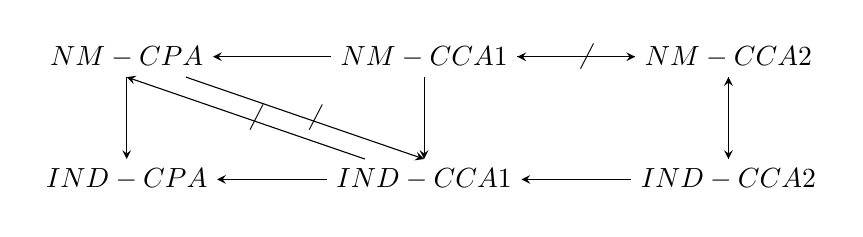
\begin{tikzpicture}
    \matrix (m) [matrix of math nodes,row sep=3em,column sep=4em,minimum width=2em]
    {
      NM-CPA & NM-CCA1 & NM-CCA2 \\
      IND-CPA & IND-CCA1 & IND-CCA2 \\
    };
    \path[-stealth]
    (m-1-2) edge node {} (m-1-1)
    (m-1-3) edge node {} (m-1-2)
    (m-2-2) edge node {} (m-2-1)
    (m-2-3) edge node {} (m-2-2)
    (m-1-1) edge node {} (m-2-1) 
    (m-1-2) edge node {} (m-2-2)
    (m-1-3) edge node {} (m-2-3)
    (m-1-1) edge node {$\not$} (m-2-2.north)
    (m-2-2) edge node {$\not$} (m-1-1.south)
    (m-2-3) edge node {} (m-1-3)
    (m-1-2) edge node {$\not$} (m-1-3);
      \end{tikzpicture}
  \caption{All relations between our defined security frameworks. See Section
    \ref{sec:allrelations} for the explanation of the arrows.}
  \label{fig:secrelations}
\end{figure}
\section{Public-Key Crypto Schemes}
\subsection{An Example: RSA}
In this section we finally illustrate how the previously discussed ideas can be
combined into a concrete scheme. However, before we can do that we must make a
brief detour to prove some results we will be using later.
\subsubsection{Mathematical set-up}
\begin{theorem}{Order}
  Let $G$ be a finite group and $g \in G$. Then, there exist positive integers
  $n$ such that $g^n = 1$. We shall call the smallest such integer the order of
  $g$, denoted $|g|$ called the \textbf{order} of $g$.
\end{theorem}
\begin{proof}
  Since $G$ is finite, there must exist $n, m \in \Nat, n \neq m$ such that
  \[
    g^n = g^m.
  \]
  Without loss of generality, we may assume $n > m$. Then, multiplying both
  sides with the inverse of $g^m$, we get
  \[
    g^{n - m } = 1.
  \]
\end{proof}
\begin{theorem}
  \label{thm:elemorderdiv}
  Let $G$ be a finite group and $g \in G$. Then, the order of $g$ divides the
  order of $G$.
\end{theorem}
\begin{proof}
  Assume that $|g| \nmid |G|$. Then, $|G| = q|g| + r$ for $q$ a non-negative
  integer and $r$ a positive integer.
\end{proof}
\begin{corollary}
  \label{cor:elemgroupordpow}
  Let $G$ be a finite group. Then,
  \[
    \forall g \in G\quad g^{|G|} = 1.
  \]
\end{corollary}
\begin{proof}
  Let $g \in G$. By Theorem \ref{thm:elemorderdiv} $|G| = q|g|$ for some $q \in
  \Nat$. Therefore,
  \[
    g^{|G|} = g^{q|g|} = (g^{|g|})^q = 1^q = 1.
  \]
\end{proof}
\begin{corollary}
  \label{thm:groupordpow}
  Let $G$ be a finite group. Then,
  \[
    \forall g \in G, p \in \Nat\quad g^p = g^{p \mod |G|}.
  \]
\end{corollary}
\begin{proof}
  \label{thm:grouppowmod}
  Let $g \in G, p \in \Nat$. Then, $p = q|G| + r$ for $q$ non-negative integer
  and $r$ a positive integer. Then, by the previous corollary $g^{|G|} = 1$, so
  \[
    g^p = g^{q|G| + r} = (g^{|G|})^qg^r = 1^qg^r= g^r = g^{p \mod |G|}.
  \]
\end{proof}
Before we may move on to the final corollary, we quickly make the following
observation:
\begin{theorem}
  Let $n \in \Nat$. The elements $x$ of $\Int_n \setminus \{0\}$ such that $\gcd(x, n) = 1$ form
  a group under multiplication with identity $1$ and inverse $a \in \Int_n$,
  where $ax + bn = 1$ from B\`ezout's identity. We denote this group by $\Int^*_n$
\end{theorem}
\begin{proof}
  It is very easy to check that the above indeed fulfils all group axioms.
\end{proof}
The order of $\Int_n$ is very important number-theoretically, so much so that it
is usually dentoted $\phi(n) = |\Int_n|$ and is called the \textbf{Euler phi-function}.
Now, we are ready to state the theorem of our interest:
\begin{theorem}{(Euler's Theorem)}\\
  \label{thm:eulersthm}
  Let $a, n \in \Nat$ such that $a < n$ and $\gcd(a, n) = 1$. Then,
  \[
    a^{\phi(n)} = 1 \mod n.
  \]
\end{theorem}
\begin{proof}
  By the above conditions $a \in \Int^*_n$. Then, the statement is a special
  case of Corollary \ref{thm:groupordpow}, where $(G, \circ) = (\Int^*_n, \times)$.
\end{proof}
\subsubsection{The Construction: RSA}
\paragraph{}
We are now ready to construct the well-known RSA scheme invented by Rivest,
Shamir and Adleman in 1978 \cite{rivest1978method}. As mentioned above, computationally secure schemes rely on
a security parameter $\lambda \in \Nat$. Increasing it will make the scheme run
slower, but will also make it more resilient.
\paragraph{Key generation}
\begin{enumerate}
\item Pick 2 primes $p, q$ such that $2^\lambda < p, q <
2^{\lambda + 1}$.
\item Calculate $N = pq$ and $\phi(N) = (p - 1)(q - 1)$.
\item Pick a number $i \in \Nat$ such that $\gcd(i, N) = 1$. Then $i \in
  \Int^*_N$.
\item Calculate $j = i^{-1}$ in $\Int^*_N$. This can be done by using the
  Extended Euclidean Algorithm to calculate $\gcd(i, \phi(N))$.
\item Output $k_\Enc = (N, i)$ and $k_\Dec = (N, j)$.
\end{enumerate}
\paragraph{Encryption}
Our message and cipher space are the binary string representations of naturals such that $m
< N$. Formally, $\M = \C = \{0, 1\}^{\lfloor {\log_2N} \rfloor}$.
\begin{enumerate}
\item Given public key $(N, i)$ and message $m \in \M$ calculate $c = m^i \mod N$.
\item Output $c$.
\end{enumerate}
\paragraph{Decryption}
\begin{enumerate}
\item Given private key $(N, j)$, and ciphertext $c \in \C$ calculate $m'''''''' = c^j \mod
  N$.
\item Output $m''''$.
\end{enumerate}
\paragraph{Correctness} To show that the above scheme is indeed a cipher, we
must show that it is correct, i.e. that
\[
  \forall (k_\Enc, k_\Dec) \in \K, \forall m \in \M\quad\text{we have}\quad
  \Dec_{k_\Dec}(\Enc_{k_\Enc}(m)) = m.
\]
To see this, let $k_\Enc = (N, i)$ and $k_\Dec = (N, j)$ such that $(k_\Enc,
k_\Dec) \in \K$ and let $m \in \M$ be arbitrary. Then,
\[
  c = \Enc_{k_\Enc}(m) = m^i \mod N.
\]
Decrypting, we get
\begin{align*}
  m' &= \Dec_{k_\Dec}(c) \\
     &= c^j \mod N \\
     &= (m^i)^j \mod N = m^{ij} \mod N \\
     &= m^{ij \mod N} \mod N \quad \text{by Corollary \ref{thm:grouppowmod}} \\
     &= m^1 \mod N \quad \text{Since $j$ is the multiplicative inverse of $i$ mod $N$ by definition}
\end{align*}
Since $m < N$ we may omit the mod $N$ on the last line. Therefore m = m' and so the scheme is correct.
\section{Homomorphic Crypto Schemes}
\paragraph{}
At this point, we start to finally focus on the topic of the dissertation:
homomorphic schemes. Intuitively, these encapsulate the idea of encrypted
comptutation over encrypted data, in sense that the adversary may at most
observe the operation take place, but both the inputs and the output of it
remain secret. In this section we give the formal definition, construct an
example scheme known as the Paillier scheme. Finally, we close with a discussion
on the limitation of homomorphic schemes.
\subsection{Definition}
\begin{definition}{Homomorphic Encryption}
  Let $\Pi = (\Gen, \Enc, \Dec)$ be a cipher with message space $\M$ and cipher
  space $\C$. Furtermore, let $(\M, \circ)$ and $(\C, \oplus)$ be groups where
  $\circ, \oplus$ are binary operations.
  We say that $\Pi$ is homomorphic iff $\forall (k_\Enc, k_\Dec) \in \K, \forall
  m_1, m_2 \in \M, c_1 = \Enc_{k_\Enc}(m_1), c_2 = \Enc_{k_\Enc}(m_2)$ we have
  \[
    m_1 \circ m_2 = \Dec_{k_\Dec}(c_1 \oplus c_2).
  \]
\end{definition}
\subsection{Paillier's Scheme}
\paragraph{}
Here we will give a concrete example of a homomorphic scheme, called the Paillier
cryptosystem, named after Pascal Paillier, who invented it in 1999
\cite{paillier1999public}. Once again, however, before we discuss the
construction of the scheme, we must familiarize ourselves with the theory upon
which it is built.
\subsection{Mathematical Set-up}
The cryptosystem is built on a particular isomorphism between two groups, that
we will be proving here. However, before we can do that, we revisit the $\phi$
function.
\begin{theorem}
  \label{thm:phiformula}
  Recall that Euler's $\phi$-function is defined as
  \[
    \phi(N) = |\{k \in \{0\hdots N - 1\} \,\,|\,\, \gcd(k, N) = 1\}|
  \]
  Assume $N = \prod_{i = 1}^n p_i^{e_i}$, for $p_i$ primes and $e_i$ naturals. Then,
  \[
    \phi(N) = \prod_{i = 1}^n p_i^{e_i - 1} (p_i - 1).
  \]
\end{theorem}
\begin{proof}
  We will present a simple counting argument using the inclusion-exclusion
  principle. That is, let $\P$ be the set of prime divisors of $N$, and
  let $\D_P$, where $P \subseteq \P$ be the set of integers
  between $0$ and $N - 1$ divisible by all primes in $P$. Formally:
  \[
    \text{For } P \subseteq \P \quad \D_P = \{n \in \{0 \hdots
    N - 1\}\,\,|\,\,p | n\,\,\forall p \in P\}.
  \]
  Then, our problem can be reformulated in the following way:
  \[
    \phi(N) = |\D_\emptyset|.
  \]
  We observe the following two simple facts: First
  \[
    |\D_P| = \frac{|N|}{\prod_{p \in P}p} = \prod_{i = 1}^n p_i^{e_i -
      1} \times \prod_{p \not\in P}p
  \]
  Second, for any $A = \{a_1, a_2, \hdots a_n\}$ integers we have
  \begin{equation}
    \label{eq:prodexpansion}
    \prod_{i = 1}^n (a_i - 1) = \sum_{i = 0}^n (-1)^i
 \sum_{\substack{B \subseteq A \\ |B| = n - i}} \prod_{a \in B}a
  \end{equation}
  This holds, because if we expand the left-hand term, then every term in the
  result will be a product of $n - k$ first terms and $k$ second terms. The
  expression on the right hand merely captures summing all possible combinations.
  By the inclusion-exclusion principle we have
  \begin{align*}
    |\D_\emptyset| &= |\{0 \hdots N-1\}| - \sum_{\substack{P \subseteq \P \\ |P| =
        1}} |\D_P| + \sum_{\substack{P \subseteq \P \\ |P| =
        2}} |\D_P| - \hdots \sum_{\substack{P \subseteq \P \\ |P| =
    |\P|}} |\D_P| \\
                   &= N + \sum_{i = 1}^n (-1)^i \sum_{\substack{P \subseteq \P \\ |P| =
    i}} |\D_P| \\
                   &= N + \sum_{i = 1}^n (-1)^i \sum_{\substack{P \subseteq \P \\ |P| =
        i}} \left(  \prod_{i = 1}^n p_i^{e_i - 1} \times \prod_{p \not\in P}p \right)\\
                   &= \prod_{i = 1}^n p_i^{e_i - 1} \left( \prod_{p\in\P}p +  \sum_{i = 1}^n (-1)^i \sum_{\substack{P \subseteq \P \\ |P| =
    i}} \prod_{p \not\in P}p \right) \quad \text{merge the product with the sum}\\
                   &= \prod_{i = 1}^n p_i^{e_i - 1} \left( \sum_{i = 0}^n (-1)^i
 \sum_{\substack{P \subseteq \P \\ |P| = n - i}} \prod_{p \in P}p \right) \quad\text{by Equation \ref{eq:prodexpansion}}\\
                   &=\prod_{i = 1}^n p_i^{e_i - 1}\prod_{p \in \P} (p - 1) = \prod_{i = 1}^n p_i^{e_i - 1}(p_i - 1).
 \end{align*}
\end{proof}
\paragraph{Note:} A much nicer proof of the above result follows from Chinese
Remainder Theorem using the fact that for $m, n \in \Nat$ where $\gcd(m, n) = 1$
we have $\phi(mn) = \phi(m)\phi(n)$, but this is outside the scope of this work. 
\begin{theorem}
  \label{thm:paillierthms}
Let $1^n$ be our security parameter. Let $p, q$ be primes such that
$|p| = |q| = n$ and $N = pq$. Then, the following hold:
\begin{enumerate}
\item $\gcd(N, \phi(N)) = 1$
\item For any $a \in \Int_{N^2}^*$ we have $(1 + N)^a = 1 + aN \mod N^2$. In
  particular, the order of $1 + N$ is $N$.
\item We have $\Int_{N^2}^* \cong \Int_{N} \times \Int_{N}^*$.
In particular, the isomorphism $f:\Int_{N} \times \Int_{N}^* \mapsto \Int_{N^2}^*$
is given by
\[
   f((a, b)) = (1 + N)^a \times b^N \quad\text{for}\,\, a \in \Int_{N}, b \in \Int_{N}^*.
\]
\end{enumerate}  
\end{theorem}
\paragraph{Claim 1:} We may assume without loss of generality, that $p > q$.
Then obviously $\gcd(p, p - 1) = 1$ and $\gcd(p, q - 1) = 1$. If $\gcd(q, p - 1)
\neq 1$, then $\gcd(q, p - 1) = q$, since $q$ is a prime. But then $p - 1 = aq$
for some $a \in \Nat$, in particular $\frac{p - 1}{2} \geq q$ from which $|p| >
|q|$, a contradiction, hence $\gcd(q, p - 1) = 1$. From this we have $\gcd(q,
\phi(N)) = 1$ and $\gcd(p, \phi(N)) = 1$ and therefore $\gcd(N, \phi(N)) = 1$.
\paragraph{Claim 2:} Expanding $(1 + N)^a$ by the binomial theorem, we get
\[
  (1 + N)^a = \sum_{i =0}^a \binom{a}{i} N^i
\]
Reducing modulo $N^2$, all terms with degree 2 or higher become 0 and the only
two terms remaining will be $1 + aN$. From this, setting $a = N$ we get $(1 +
N)^N = 1$, and this is the smallest possible positive integer.
\paragraph{Claim 3:}
For clarity, we shall follow the notation of \cite{katz2014introduction} and
write
\[
  (a, b) \leftrightarrow x \Leftrightarrow f((a,b)) = x
\]
\begin{proof}
  We shall break down the proof into the following steps:
  \begin{enumerate}[i.]
  \item Show $f$ is a bijection.
  \item Show $f$ is a homomorphism.
  \end{enumerate}
  \paragraph{Claim 3.i} We first note the following:
  \[
    |\Int_{N}| = N = pq,\quad
    |\Int_{N}^*| = \phi(N) = (p - 1)(q - 1),\quad
    |\Int_{N^2}^*| = \phi(N^2) = pq(p - 1)(q - 1),
  \]
  where the last two equalities hold by Theorem \ref{thm:phiformula}.
  This means that since $|\Int_{N} \times \Int_{N}^*| = |\Int_{N}|
  \times |\Int_{N}^*|$ we have $|\Int_{N} \times \Int_{N}^*| = |\Int_{N^2}^*|$.
  Hence, we only need to show that $f$ is a injection to show that it is a bijection.
  \paragraph{}
  Therefore, let $f((a_1, b_1)) = f((a_2, b_2))$ for some $(a_1, b_1), (a_2,
  b_2) \in \Int_{N} \times \Int_{N}^*$. Then,
  \[
    (1 + N)^{a_1}\times b_1^N = (1 + N)^{a_2}\times b_2^N\mod N^2
  \]
  Then, since we have inverses in both $\Int_N$ and $\Int_N^*$, we have
  \[
    (1 + N)^{a_1 - a_2}\times (b_1b_2^{-1})^N = 1 \mod N^2
  \]
  Since $b_1, b_2 \in \Int_N^*$, raising both sides to the power of $\phi(N)$,
  we get
  \begin{align*}
    (1 + N)^{\phi(N)(a_1 - a_2)} \times ((b_1b_2^{-1})^{\phi(N)})^N &= 1 \mod N^2 \\
    (1 + N)^{\phi(N)(a_1 - a_2)}  &= 1 \mod N^2\quad\text{by Corollary \ref{cor:elemgroupordpow}}
  \end{align*}
  Then, since by Claim 1 $\gcd(N, \phi(N)) = 1$, it must be the case that $(1 +
  N)^{a_1 - a_2} = (1 + (a_1 - a_2)N) = 1 \mod N^2$. Hence $a_1 - a_2 = 0 \mod N^2$
  and since $a_1, a_2 \in \Int_N$ the above is an equality, from which we have
  $a_1 = a_2$.
  \paragraph{} Going back to our initial formula, now simplifying by the terms
  involving the $a$s:
  \[
    b_1^N = b_2^N \mod N^2.
  \]
  Since $b_1, b_2 \in \Int_N^*$ we have $b_1, b_2\in \Int_{N^2}^*$. But
  exponentiation in finite groups is a bijection, hence $b_1 = b_2 \mod N^2$.
  Again, since $b_1, b_2 < N$, it is actually an equality. Thus $f$ is
  injective, and hence bijective.
  \paragraph{Claim 3.ii} Let $a_1, a_2 \in \Int_N$ and $b_1, b_2 \in \Int_N^*$. We need to show that
  \[
    f((a_1, b_1)) \times f((a_2, b_2)) = f((a_1 + a_2), (b_1b_2)).
  \]
  We note that the multiplication on the left-hand side is carried out modulo
  $N^2$, whereas the addition and multiplication on the right-hand side is done
  modulo $N$. We will begin with
  \begin{align*}
    (1 + N)^{a_1}b_1^N(1 + N)^{a_2}b_2^N &= (1 + N)^{a_1 + a_2}(b_1b_2)^N \mod N^2 \\
                                         &= (1 + N)^{[a_1 + a_2 \mod N]}(b_1b_2)^N \mod N^2 \quad \text{by Claim 2 and Theorem \ref{thm:grouppowmod}}
  \end{align*}
  The addition is now carried out modulo $N$, but there is some more work with
  the multiplication. Let $b_1b_2 = \gamma N + r$ where $0 \leq \gamma$ and $0 <
  r \leq N$. Note that $r \neq 0$, since that would mean $b_1b_2$ is divisible
  by $N$, but it is not since it is in $\Int_N^*$. Then, by the Binomial
  Theorem, we have
  \begin{align*}
    (b_1b_2)^N &= (\gamma N + r)^N \\
               &= \sum_{i = 0}^N \binom{N}{i}(\gamma N)^ir^i \\
               &= r^N \mod N
  \end{align*}
  This means that $(b_1b_2)^N$ is an Nth power modulo $N$, and hence $f$ is a
  homomorphism. \\
  By Claim 3.i and Claim.ii, $f$ is an isomorphism.
\end{proof}
Finally, we look at the particular set of elements used in Paillier's scheme:
$N$th residues.
\begin{definition}{Nth residue:} Let $G$ be a group and let $x, y \in G$. Then, we call $x$
  an Nth residue, if $x^N = y$, and write $x \in \texttt{Res}(G)$.
\end{definition}
We now characterise Nth residues in $\Int_{N^2}^*$.
\begin{theorem}
  Let $x \in \texttt{Res}(\Int_{N^2}^*)$ be an Nth residue. Then, $\exists b \in
  \Int_N^*$ such that
  \[
    x \leftrightarrow (0, b),
  \]
  and thus
  \[
    \texttt{Res}(\Int_{N^2}^*) = \{b \,\,|\,\, b \in \Int_N^*\}.
  \]
\end{theorem}
\begin{proof}
  We will construct a generic Nth residue. Let $a \in \Int_N$ and $b \in
  \Int_N^*$. By Claim 1, $\gcd(N, \phi(N)) = 1$, hence $N$ has a multiplicative
  inverse mod $\phi(N)$. Call this inverse $d = N^{-1}$. Then, $b^d$ is also in $\Int_N^*$. Then, let $x \in \Int_{N^2}^*$ such
  that
  \[
    x \leftrightarrow (a, b^d).
  \] 
  Note, that since $a$ and $b$ were arbitrary and $f$ is an isomorphism, every
  element of $\Int_{N^2}^*$ can be written in the above form. Raising both sides
  to the Nth power, we get
  \begin{align*}
    x^N &\leftrightarrow (a, b^d)^N \\
        &\leftrightarrow (aN \mod N, b^{dN} \mod N) \\
        &\leftrightarrow (0, b).
  \end{align*}
\end{proof}
\paragraph{} We also note that it is easy to see from the above that there are
precisely $N$ elements mapping to the same residue, since all elements of the
form $(a, b^d)$ map to $(0, b)$, and since $a\in \Int_N$, there are $N$ choices
for $a$.
\paragraph{} Now, we have all the tools required to construct the scheme.
\subsection{The Construction: Paillier Cryptoscheme}
\paragraph{Key Generation}
Pick two primes of length equal to the security parameter, i.e. $p, q$ primes,
such that $|p| = |q| = |\lambda|$. Calculate $N = pq$, $N^2$ and $\phi(N) = (p -
1)(q - 1)$.
Then output $pk = N^2$ and $sk = \phi(N)$.
\paragraph{Encryption}
Let $m$ be the message we wish to encrypt. Pick a uniform $(0, r) \in
\Int_{N^2}^*$. Then output the ciphertext $c = (m, 1) \times (0, r) = (m, r)$.
\paragraph{Decryption} 
Let $c$ be the ciphertext we wish to decrypt. First, let $\hat{c} = c^{\phi(N)}
\mod N^2$. Then, calculate $m' = \frac{(\hat{c} - 1)}{N} \times \phi(N)^{-1} \mod N$.
Output $m'$.
\paragraph{Correctness}
Let $(pk, sk)$ be the key $\Gen$ generates, with $pk = N^2$, for some $N = pq$
primes and $sk = \phi(N)$. Let$m$ be the message we encrypt and $c =
\Enc_{pk}(m) =(m, r)$ for some uniformly random $r$. Then
\begin{align*}
  \hat{c} &= c^{\phi(N)} = (m, r)^{\phi(N)} = (\phi(N)m, r^{\phi(N)}) \\
          &= (\phi(N)m, 1) \quad \text{by Corollary \ref{cor:elemgroupordpow}}\\
          &\leftrightarrow (1 + N)^{\phi(N)m} \mod N^2 \quad \text{by Theorem \ref{thm:paillierthms} part 2}\\
          &= (1 + \phi(N)mN) \mod N^2.
\end{align*}
Then, we have
\begin{align*}
  \Dec_{sk}(c) &= \frac{\hat{c} - 1}{N} \times \phi(N)^{-1} \mod N\\
               &= \frac{(1 + \phi(N)mN) - 1}{N} \times \phi(N)^{-1} \mod N\\
               &= \frac{\phi(N)mN}{N}\times \phi(N)^{-1} \mod N\\
               &= \phi(N)m \times \phi(N)^{-1} \mod N \\
               &= m \mod N. \\
               &= m \quad \text{since } m < N.
\end{align*}
Thus, $m = \Enc_{pk}(\Dec_{sk}(m))$, and so the scheme is correct, and therefore
a cipher.
\section{Lattices}
\paragraph{}
In the previous section we have seen the motivating idea behind Gentry's scheme:
encrypted computation. In this section, we aim to provide a brief introduction
to the tool that helped the scheme come to life: lattices. We will define what a
lattice is and see some key definitions and theorems. We will close the section
with a construction of a simple lattice-based crypto scheme to illustrate how
the theory may be used to construct secure schemes with the appropriate choice
of a trapdoor.
\subsection{Mathematical Set-up I: Introduction to Lattices}
\paragraph{} We shall begin by a basic introduction to lattices in general, then
turn our attention to computational problems involving lattices. In the
following section, we construct a very simple cryptosystem that relies on the
ideas we explore here.
\begin{definition}{(Finite dimensional) Lattice:}
  Let $V = \Reals^n$ be the $n$-dimensional Euclidean space, and $B = \{\vec{v}_1,
  \vec{v}_2, \hdots, \vec{v}_n\}$ be a basis for $V$. Then, the \textbf{lattice generated by $B$} is the set
  \[
    \L(B) = \{\alpha_1\vec{v}_1 + \alpha_2\vec{v}_2 + \hdots \alpha_n\vec{v}_n\,\,|\,\, \vec{v}_i \in B,
    \alpha_i \in \Int\}.
  \]
  Then $B$ is also called the basis of the lattice $\L$.
\end{definition}
\begin{definition}{Fundamental Domain}
  Let $\L$ be a lattice with basis $B = \{\vec{v}_1, \vec{v}_2, \hdots, \vec{v}_n\}$. Then, the
  \textbf{fundamental domain of $\L$ with respect to $B$} is
  \[
    \F_B = \{t_1\vec{v}_1 + t_2\vec{v}_2 + \hdots + t_n\vec{v}_n \,\,|\,\, \vec{v}_i \in B, t_i \in [0,
    1)\} \subseteq \Reals^n.
  \]
\end{definition}
The following theorem is key for cryptographic application of lattices:
\begin{theorem}
  Let $\L$ be a lattice with basis $B$. Then $\F_B$ tessalates $\Reals^n$
  without overlap. Formally, let $x \in \Reals^n$. Then there exists a unique $\ell \in \L$
  and $f \in \F_B$ such that
\[
  x = \ell + f.
\]
\end{theorem}
\begin{proof}
  Let $x \in \Reals^n$ be arbitrary. Since $B = \{ \vec{v}_1, \hdots, \vec{v}_n \}$ is a basis for $\Reals^n$, there
  is a unique combination of its vectors that give $x$, i.e. there exist unique
  reals $a_1, \hdots, a_n$ such that
  \[
    x = a_1\vec{v}_1 + \hdots + a_n\vec{v}_n.
  \]
  For all $i$ let $\alpha_i = \lfloor a_i \rfloor$ and $t_i = a_i - \lfloor a_i
  \rfloor$. We note that by the definition of the floor function, $0 \leq t_i <
  1$ for all $i$. Then, letting $\ell = \sum_{i = 1}^n \alpha_i\vec{v}_i$ and $f
  = \sum_{i = 1}^n t_i\vec{v}_i$, we clearly have $\ell \in \L$ and $f \in
  \F_B$. Now, from the above equation we get
  \begin{align*}
    x &= (\alpha_1 + t_1)\vec{v}_1 + \hdots (\alpha_n + t_n)\vec{v}_n \\
      &= \alpha_1\vec{v}_1 + \hdots + \alpha_n\vec{v}_n + t_1\vec{v}_1 + \hdots + t_n\vec{v}_n \\
      &= \ell + f \quad \text{as required.}
  \end{align*}
\end{proof}
The following result is an important result about lattices.
\begin{theorem}
  Let $\L$ be a lattice with bases $B_1$ and $B_2$. Then $\det(B_1) = \det(B_2)$
  and is called the \textbf{covolume} of $\L$, denoted Vol($\L$).
\end{theorem}
\begin{proof}
\end{proof}
\begin{theorem}
  Let $\L$ be a lattice with basis $B = \{\vec{v}_1, \vec{v}_2, \hdots \vec{v}_n\}$. Then
\[
  \text{Vol}(\L) \leq \norm{\vec{v}_1}\cdot\norm{\vec{v}_2}\cdots\norm{\vec{v}_n}.
\]
\end{theorem}
\begin{proof}
\end{proof}
Based on the above theorem, we will make the following definition:
\begin{definition}{Hadamard Ratio}
  Let $\L$ and $B$ as in the theorem above. Then, the \textbf{Hadamard ratio of $B$}
  is defined as
  \[
    \H(B) = \left( \frac{\text{Vol}(\L)}{\norm{\vec{v}_1}\cdot\norm{\vec{v}_2}\cdots\norm{\vec{v}_n}} \right)^{\frac1n}.
  \]
\end{definition}
We note that by the above theorem $0 < \H(B) \leq 1$.
\subsection{Mathematical Set-up II: Computational Lattice Problems}
SVP
CVP
Babai's algorithm
\subsection{The Construction: GGH}
\paragraph{Key Generation}
\paragraph{Encryption}
\paragraph{Decryption}
\paragraph{Correctness}
\section{Fully Homomorphic Encryption}
\subsection{Dr Craig Gentry's Scheme}

\printbibliography

\end{document}